% LaTeX Jeopardy Game
% by Braden Licastro
% 2 Oct 2014
%
% A modification of beamer latex template by DCMST
% on StackExchange for Tex.
%
% NOTES:
%  This game MUST be compiled using PDFLaTeX
%  This game can ONLY be played in Adobe Reader due to the javascript links (ocgx)
%  You must only use the mouse to click the buttons, any other interaction breaks the game
%  You must hide the prize before going home due to LaTeX limitations
%  You must have fun, or else.

\NeedsTeXFormat{LaTeX2e}
\documentclass{beamer}
\usepackage[]{autojeopardy} % Accepts no parameters

\usepackage{amssymb} % Math symbols

\begin{document}
\begin{frame}
\hypertarget{home}{}
\vspace*{-.5cm}
    \subjects{Logic}{Professors}{The Major}{Calculus I}{``Category 5''}
    \prizes
\end{frame}

% Section 1 Question 100
\content                       % 4 arguments
    {s1-100}                     % question internal identifier
    {Logic}                          % subject number
    {100 POINTS}{                       % question prize
        \begin{textarea}[]         % question/answer content
        \only<1>{
            I am an odd number. Take away one letter and I become even.
        }
        \only<2>{
            What is seven? (Take away the `s' and it becomes `even')
        }
        \end{textarea}
    }
% Section 1 Question 200
\content
    {s1-200}                     % question internal identifier
    {Logic}                          % subject number
    {200 POINTS}{                       % question prize
        \begin{textarea}[]         % question/answer content
        \only<1>{
            Among the assertions made in this problem there are three errors.\\
            What are they?
			\begin{enumerate}[(a)]
            	\item $2 + 2 = 4$
            	\item $4 \div \frac{1}{2} = 2$
            	\item $3\frac{1}{5} \times 3\frac{1}{8} = 10$
            	\item $7 - (-4) = 11$
            	\item $-10 (6 - 6) = -10$
            \end{enumerate}
        }
        \only<2>{
            What are \textbf{(b)}, \textbf{(e)} and the fact that there aren't three errors?
        }
        \end{textarea}
    }
% Section 1 Question 300
\content
    {s1-300}                     % question internal identifier
    {Logic}                          % subject number
    {300 POINTS}{                       % question prize
        \begin{textarea}[]         % question/answer content
        \only<1>{
            The next symbol in this sequence.\\
            
\includegraphics[scale=1.5]{s1q300}
        }
        \only<2>{
            What is 
\includegraphics[scale=.25]{s1a300}?
        }
        \end{textarea}
    }
% Section 1 Question 400
\content
    {s1-400}                     % question internal identifier
    {Logic}                          % subject number
    {400 POINTS}{                       % question prize
        \begin{textarea}[]         % question/answer content
        \only<1>{
            A logician vacationing in the South Seas finds himself on an island inhabited by the two proverbial tribes of liars and truth-tellers. Members of one tribe always tell the truth, members of the other always lie. He comes to a fork in the road and has to ask a native bystander which branch he should take to reach a village. He has no way of telling whether the native is a truth-teller or a liar. The logician thinks a moment, then asks \textit{one} question only. From the reply he knows which road to take. What did he ask?
        }
        \only<2>{
            ``If I were to ask you if this road leads to the village, would you say yes?''
        }
        \end{textarea}
    }
% Section 1 Question 500
\content
    {s1-500}                     % question internal identifier
    {Logic}                          % subject number
    {500 POINTS}{                       % question prize
        \begin{textarea}[]         % question/answer content
        \only<1>{
            An intelligent horse learns arithmetic, algebra, geometry, and trigonometry but is unable to understand the Cartesian coordinates of the analytic geometry. What proverb does this suggest?
        }
        \only<2>{
            Proverb:\\
            \textit{Do not put Descartes before the horse.}
        }
        \end{textarea}
    }


% Section 2 Question 100
\content
    {s2-100}                     % question internal identifier
    {Professors}                          % subject number
    {100 POINTS}{                       % question prize
        \begin{textarea}[]         % question/answer content
        \only<1>{
            The current Department Chair.
        }
        \only<2>{
            Who is Professor Lakins?
        }
        \end{textarea}
    }
% Section 2 Question 200
\content
    {s2-200}                     % question internal identifier
    {Professors}                          % subject number
    {200 POINTS}{                       % question prize
        \begin{textarea}[]         % question/answer content
        \only<1>{
            The Actuarial Adviser and has a PHD from Yale.
        }
        \only<2>{
            Who is Dr. LoBello?
        }
        \end{textarea}
    }
% Section 2 Question 300
\content
    {s2-300}                     % question internal identifier
    {Professors}                          % subject number
    {300 POINTS}{                       % question prize
        \begin{textarea}[]         % question/answer content
        \only<1>{
            The Engineering Liaison.
        }
        \only<2>{
            Who is Professor Weir?
        }
        \end{textarea}
    }
% Section 2 Question 400
\content
    {s2-400}                     % question internal identifier
    {Professors}                          % subject number
    {400 POINTS}{                       % question prize
        \begin{textarea}[]         % question/answer content
        \only<1>{
            The Dimensions Club Adviser.
        }
        \only<2>{
            Who is Professor Werner?
        }
        \end{textarea}
    }
% Section 2 Question 500
\content
    {s2-500}                     % question internal identifier
    {Professors}                          % subject number
    {500 POINTS}{                       % question prize
        \begin{textarea}[]         % question/answer content
        \only<1>{
            The $\Pi$ME Adviser.
        }
        \only<2>{
            Who is Professor Carswell?
        }
        \end{textarea}
    }
    

% Section 3 Question 100
\content
    {s3-100}                     % question internal identifier
    {The Major}                          % subject number
    {100 POINTS}{                       % question prize
        \begin{textarea}[]         % question/answer content
        \only<1>{
            Mathematics is in this division.
        }
        \only<2>{
            What is Natural Science?
        }
        \end{textarea}
    }
% Section 3 Question 200
\content
    {s3-200}                     % question internal identifier
    {The Major}                          % subject number
    {200 POINTS}{                       % question prize
        \begin{textarea}[]         % question/answer content
        \only<1>{
            The number of credits required for the Math major at Allegheny.
        }
        \only<2>{
            What is 43?
        }
        \end{textarea}
    }
% Section 3 Question 300
\content
    {s3-300}                     % question internal identifier
    {The Major}                          % subject number
    {300 POINTS}{                       % question prize
        \begin{textarea}[]         % question/answer content
        \only<1>{
            The number of credits required for a Math minor at Allegheny.
        }
        \only<2>{
            What is 20?
        }
        \end{textarea}
    }
% Section 3 Question 400
\content
    {s3-400}                     % question internal identifier
    {The Major}                          % subject number
    {400 POINTS}{                       % question prize
        \begin{textarea}[]         % question/answer content
        \only<1>{
            The required 300 level courses for a Math Major.
        }
        \only<2>{
			Linear Algebra (320)\\
        	Algebraic Structures I (325)\\
        	Introduction to Analysis (340)
        }
        \end{textarea}
    }
% Section 3 Question 500
\content
    {s3-500}                     % question internal identifier
    {The Major}                          % subject number
    {500 POINTS}{                       % question prize
        \begin{textarea}[]         % question/answer content
        \only<1>{
            The 400 level Math courses.
        }
        \only<2>{
            Topology (400)\\
            Algebraic Structures II (425)\\
            Real Analysis (440)
        }
        \end{textarea}
    }


% Section 4 Question 100
\content
    {s4-100}                     % question internal identifier
    {Calculus I}                         % subject number
    {100 POINTS}{                       % question prize
        \begin{textarea}[]         % question/answer content
        \only<1>{
            {\huge $\int \frac{dx}{5-3x}$}
        }
        \only<2>{
            {\Large $-\frac{1}{3} ln \lvert 5-3x \rvert + C$}
        }
        \end{textarea}
    }
% Section 4 Question 200
\content
    {s4-200}                     % question internal identifier
    {Calculus I}                         % subject number
    {200 POINTS}{                       % question prize
        \begin{textarea}[]         % question/answer content
        \only<1>{
            {\Large $\lim_{x \to \frac{\pi}{2}}\frac{1 - \sin{(x)}}{\cos{(x)}^2}$}
        }
        \only<2>{
            {\huge $\frac{1}{2}$}
        }
        \end{textarea}
    }
% Section 4 Question 300
\content
    {s4-300}                     % question internal identifier
    {Calculus I}                         % subject number
    {300 POINTS}{                       % question prize
        \begin{textarea}[]         % question/answer content
        \only<1>{
            The values of $a$ and $b$ such that the line $2x + y = b$ is \\
            tangent to the parabola $y = ax^2$ when $x=2$.
        }
        \only<2>{
            {\Large $a = -\frac{1}{2}$\\
            $b = 2$}
        }
        \end{textarea}
    }
% Section 4 Question 400
\content
    {s4-400}                     % question internal identifier
    {Calculus I}                         % subject number
    {400 POINTS}{                       % question prize
        \begin{textarea}[]         % question/answer content
        \only<1>{
            The equation of the line tangent to \\$2(x^2 + y^2)^2 = 25(x^2 - y^2)$ at the point $(3,1)$.
        }
        \only<2>{
			{\Large $y = \frac{40}{13} - \frac{9x}{13}$}\\
			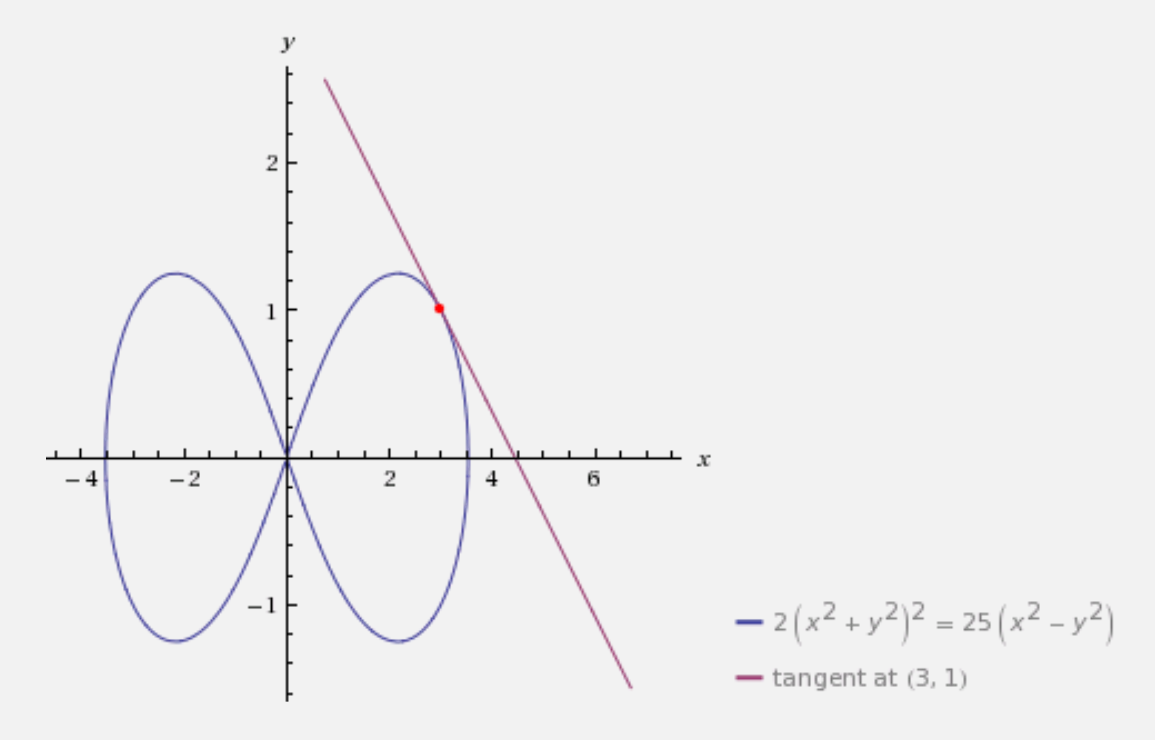
\includegraphics[scale=.225]{s4-400}
			
        }
        \end{textarea}
    }
% Section 4 Question 500
\content
    {s4-500}                     % question internal identifier
    {Calculus I}                         % subject number
    {500 POINTS}{                       % question prize
        \begin{textarea}[]         % question/answer content
        \only<1>{
            {\Large $\int \frac{3x^3 - 17x^2 + 36x - 35}{x^2 - 4x + 4}dx$}
        }
        \only<2>{
            {\Large $\frac{3}{2}x^2 - 5x + 4ln \lvert x - 2 \rvert + \frac{7}{x - 2} + C$}
        }
        \end{textarea}
    }


% Section 5 Question 100
\content
    {s5-100}                     % question internal identifier
    {``Category 5''}                         % subject number
    {100 POINTS}{                       % question prize
        \begin{textarea}[]         % question/answer content
        \only<1>{
            The year in which Allegheny College was founded.
        }
        \only<2>{
            What is 1815?
        }
        \end{textarea}
    }
% Section 5 Question 200
\content
    {s5-200}                     % question internal identifier
    {``Category 5''}                         % subject number
    {200 POINTS}{                       % question prize
        \begin{textarea}[]         % question/answer content
        \only<1>{
            The course number of the Mathematics Junior Seminar.
        }
        \only<2>{
            What is 585?
        }
        \end{textarea}
    }
% Section 5 Question 300
\content
    {s5-300}                     % question internal identifier
    {``Category 5''}                         % subject number
    {300 POINTS}{                       % question prize
        \begin{textarea}[]         % question/answer content
        \only<1>{
            The 6th Fibonacci number.
        }
        \only<2>{
            What is $5$?
        }
        \end{textarea}
    }
% Section 5 Question 400
\content
    {s5-400}                     % question internal identifier
    {``Category 5''}                         % subject number
    {400 POINTS}{                       % question prize
        \begin{textarea}[]         % question/answer content
        \only<1>{
            The number that always results from the following:
            \begin{enumerate}
            	\item Choose any number.
            	\item Add the next highest number to that number.
            	\item Add 9.
            	\item Divide by 2.
            	\item Subtract the original number.
            \end{enumerate}
        }
        \only<2>{
            What is $5$?
        }
        \end{textarea}
    }
% Section 5 Question 500
\content
    {s5-500}                     % question internal identifier
    {``Category 5''}                         % subject number
    {500 POINTS}{                       % question prize
        \begin{textarea}[]         % question/answer content
        \only<1>{
            The number of times can you take $5$ from $25$.
        }
        \only<2>{
            What is $1$? (Then it becomes $20$)
        }
        \end{textarea}
    }
\end{document}